\selectlanguage{english}
\def\<#1>{\textit{#1}}


\chapter{Introduction}
\section{Overview}

In 1965, Moore predicted, based on observations, that the number of transistors on integrated circuits will double approximately every two years. This was the case for many years after that, with the industry pushing hardware performance forward to meet that goal. Advancements in transistor technology made it possible to integrate more of them in the same silicon chip. Their frequency also increased, presumably doubled every 18 months. At the same time, emerging architecture techniques made it possible to further exploit the continuously increasing cpu power. The use of deeper pipelines superscalar architectures made it possible to increase the operation throughput. Out of order execution and branch predictors helped to make sure that most of the available transistors are utilized, at any given point of the execution. Moreover, hardware manufacturers were able to keep pushing for better performance, without worrying about memory consumption. They were able to achieve higher frequencies fore more transistors, by reducing the voltage supply needed, thus keeping power consumption at controlled levels. In the meantime, cache hierarchies  grew bigger and faster to meet the demands of CPU All those factors made it possible to keep a steady rate of increase in computing power, without any demand for new programming models.

That staggering rate of advancement reached a peak around 2004. At that point, manufacturers were not able to keep making transistors smaller and faster, without sacrificing power consumption. At the same time, memory performance was now too small compared to CPU frequencies, creating and unbridgeable CPU -  memory gap. In order to meet the increasing demands for computer power, computer science shifted towards multicore CPUs. After that point, improvements in performance were no longer achieved exclusively by advancements in architecture, but required fundamental software support. The excess of cores and transistors would mean nothing, if the overlaying software was not able to effectively break execution path down to independent path that could be run in parallel. From user applications, to compilers and operating systems, software needed to be redesigned in way that could exploit the extra cores and the available architecture. Nowadays, the demand for multicore CPUs is no longer an exclusive characteristic of super computers and data centers, but has become rather mainstream, entering the field of desktop computers and embedded systems. Over that time, parallel software techniques have made great steps of progress towards a more efficient utilization of every aspect of modern computer architectures. Despite that progress, parallel programming continues to be a challenging task, and a field of ongoing research.

\section{Flynn's taxonomy}
According to Michael J. Flynn, computer architectures are classified in 4 different categories, according to their instruction and data stream. 

%bulets here

Single Instruction Single Data stream (SISD). 
	A sequential architecture that employs a single processing unit, executing over a single data stream, one operation at a time. 

Single Instruction Multiple Data streams (SIMD).
	An computer  that executes the same command over multiple data streams. An example of such an architecture are Graphic Processor Units (GPUs).

Multiple Instruction Single Data streams(MISD).
	A computer where different instructions are executed on the same data stream. This architecture is quite uncommon, and in most cases it is user for false tolerance. An example is an airplane guiding system, where several routines are used and must reach a consensus.

Multiple Instruction Multiple Data streams(MIMD).
	Multiple autonomous processors execute different instructions on different data. Multicore and Distributed Systems are MIMD machines.

%eikona apo wiki http://en.wikipedia.org/wiki/Flynn%27s_taxonomy

\begin{figure}
 \centering
  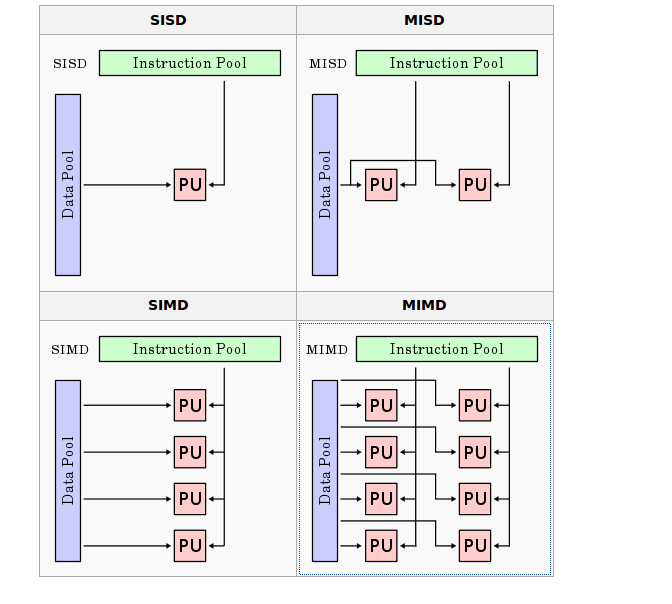
\includegraphics[scale=0.4]{flynsTaxonomy.png}
\caption{Flynn's taxonomy}
\label{Flynn's taxonomy}
\end{figure}

MIMD machines are further classified into 3 categories, according to their address space:

\subsection{shared memory}

In shared memory architectures, every processor has its own hierarchy of cache memory and all processors share the same main memory. Interconnection between processors and memory is typically done through a memory bus, but more sophisticated interconnection networks can be used. Access to memory can take the same amount of time for all processors( Uniform Memory Access -UMA ) or can vary depending on the processor and the memory location( Non Uniform Memory Access) . Non Uniform Memory Access will make memory sharing between adjacent processors fast and reduce bus congestion, but varying access time may make analysis difficult. 

%eikona gia shared memory apo diafanies https://dl-web.dropbox.com/get/SharewithCostas/Lectures/pps-parallel-programming-lec1-Fall2013.pdf?_subject_uid=122896110&w=AAB_Fj7mtgIBvGR3UK6To-ohkGaXP7AKZ7vv1mdzT95Msw

\begin{figure}
 \centering
  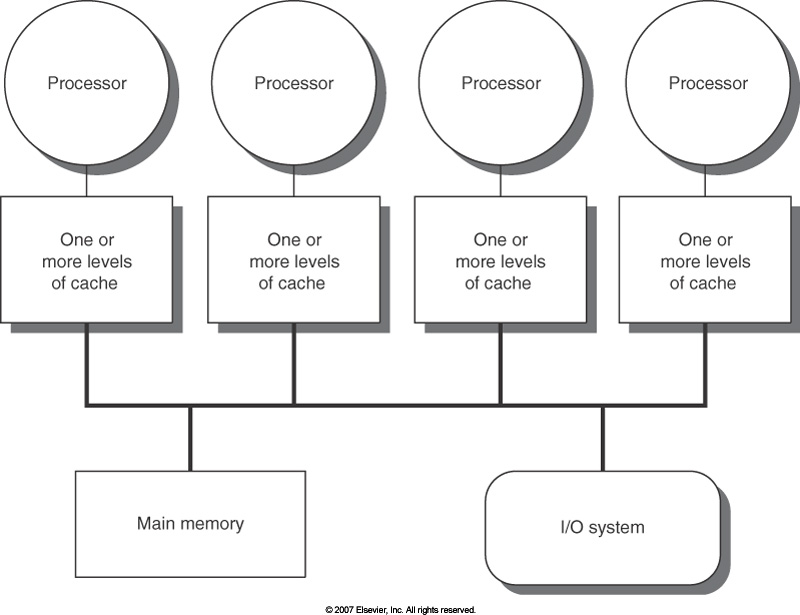
\includegraphics[scale=0.4]{shared_memory.jpg}
\caption{Shared memory Architecture}
\label{Shared memory architecture}
\end{figure}

 All working threads work on the same address space and accessing a memory location previously modified by another processor can be as simple as an access to any other variable. This makes programming in shared memory architectures seem easy, but concurrent access from different processors on the same memory location can lead to unexpected results if not a synchronization scheme is not used. Moreover, shared memory architectures wont typically scale beyond a few thousand nodes, because the bush and memory bandwidth cannot keep up with the increased traffic.

\subsection{Distributed memory}

In distributed memory architectures, every processor has it's own cache and local memory, and it has access only to that memory hierarchy.  All processors are connected on an intercontection network(Ethernet, Mirinet), consist of complex switching topologies. Communication is done using messages from processor to processor and usually being served by memory controller with direct memory access(DMA). Accessing data stored on memory outside the processor, may require several messages to be past between nodes.

%eikona gia distributed

\begin{figure}
 \centering
  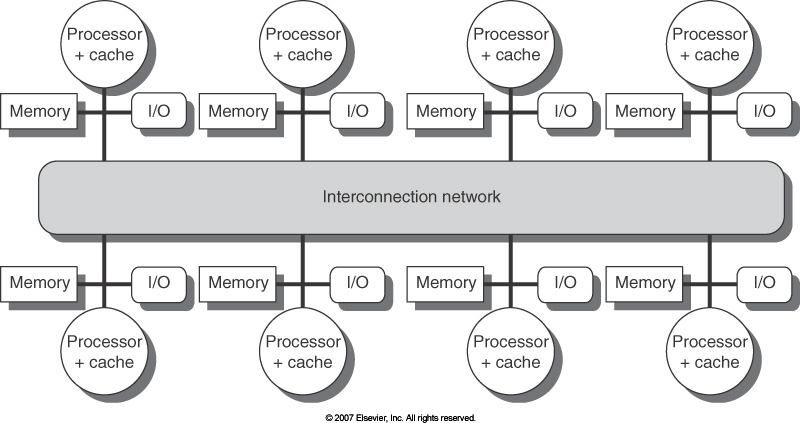
\includegraphics[scale=0.4]{distributed_memory.jpg}
\caption{Distributed memory Architecture}
\label{Distributed memory architecture}
\end{figure}
Programming in a distributed memory environment can be quite challenged, because memory locations needed by a program may not be accessible locally but have to be requested in advance. Efficient parallelization over distributed memory, requires understanding the memory dependencies of the program ability to effectively distribute memory in advance in a way that will minimize communication between distant processes. However, distributed memory can achieve far greater scalability than shared memory, up to thousands of node that can be dynamically inserted and removed from the network.

\subsection{Hybrid Memory}

In a hybrid memory architecture, a groups of processors share a common local memory and, possibly some cache levels, similar to the shared memory architecture, whereas these groups of processors communicate with each other over a  an interconnection network. This a typical topology used in clusters, where several processor share a common address space and create nodes that can be inserted in the interconnection network.

\begin{figure}
 \centering
  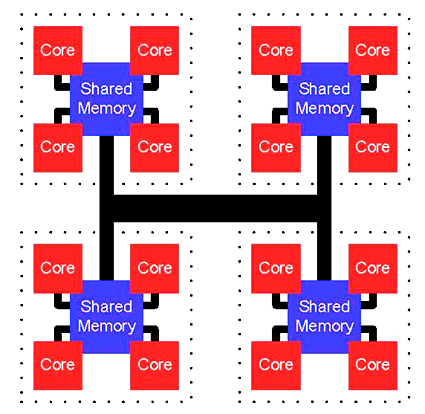
\includegraphics[scale=1.5]{hybrid_memory.jpg}
\caption{Hybrid memory Architecture}
\label{Hybrid memory architecture}
\end{figure}


\section{Synchronization}

In parallel applications, threads will eventually need to communicate with each other or perform operations on a common data structure. In the shared memory model where every shared variable is easily accessible, it would be tempting to simply modify the shared memory as if threads were running in isolation, each with access to its own memory space. This would be entirely wrong since synchronizing concurrent accesses on shared memory locations is extremely important in parallel programming. The next figure shows a simple example of how the absence of synchronized access on a counter leads to inconsistencies. The counter is incremented once by every one of the two threads, but due to the patter of operations executed, it is eventually incremented only once.

\begin{lstlisting}
	
Thread1                          Thread2

                                 var2 = counter
var1 = counter	

                                 var2 = var2 +1
                                 counter = var2

var1 = var1 +1
counter = var1

\end{lstlisting}

This problem cannot be solved with out hardware support, specifically atomic primitives that will ensure that an operation will be executed without being interrupted by a concurrent thread.  With the use of Fetch -And-Inc, incrementing a shared variable can be implemented safely, at the extra cost of locking  the memory bus until the variable is read and incremented. Other useful atomic operations, provided in most systems, are Test And Set(TAS) and Compare And Swap(CAS). Test and Set will atomically set a variable to 1 and return its previous value. Compare Snd Swap will compare the value store at a memory location with a giver value and only if they are equall, CAS will update that location to a new given value and return true. If not the operation will fail.

\section{Memory consistency}

Even if some operations can be executed atomically, the order between operations is not always guaranteed, and operations issued concurrently by many processors may actually take effect in an oder that cannot be determined in advance. In this way, no guaranteed ordering can be assumed when writing parallel programs. In an even more relaxed model, it is even possible for operations on the same core to be rearranged by the compiler or the processing unit, for various performance reasons. In that case, memory barriers can be used to make sure that operations all operations before the barrier have been completed.
\section{Synchronization And Progress}

Synchronization scheme in a parallel program  can be classified in one of three categories : blocking, lock-free and wait-free synchronization.

Blocking approaches, usually use mutual exclusion to keep only one thread to access the critical section at a time. Lock-free approaches allow several threads to access the same data and introduce overheads mostly when there are actual conflicts. Wait-free approaches guarantee that every thread will finish it's operation within a finite number of steps, although that number can be high, and are better used in real-time applications where a maximum operation latency must not be surpassed. 
 
 \begin{figure}

 \centering

  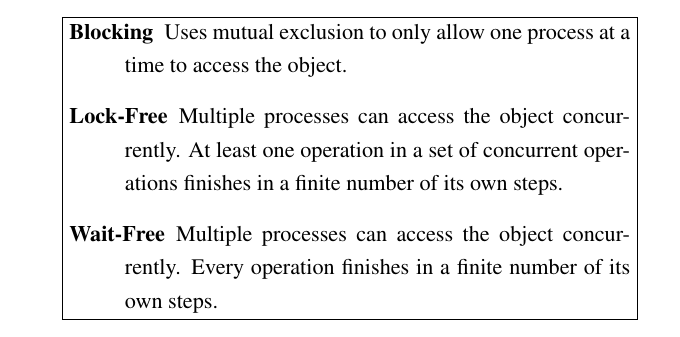
\includegraphics[scale=0.5]{progress_gar.png}

\caption{Synchronization scheme classification}

\label{progress_gar}

\end{figure}


\subsection{Blocking Synchronization}

Most of the times, blocking synchronization is achieved with the use of semaphores and locks. Almost all locks use a Test-And-Set atomic primitive to set a memory location. If that memory location is set,  and the thread that sets that location form 0 to 1 is considered as the lock owner. The use of a lock over a section of code is the easiest way to ensure that only one thread will access that section of code (critical section) at a given time.

In it's simplest form, setting a lock consists of  continuously executing TAS on the same memory location until the value return( the value in the memory location before setting it) is zero. This will cause heavy bus traffic, since every TAS will lock the buss until it is executed, along with heavy cache coherence protocol traffic, since every TAS is essentially a write that will invalidate all other copies of the lock, including the owner's. For this reason , a basic improvement is the uses of a Test and Test And Set (TTAS) lock, where the value of the lock is first read locally and a thread will attempt to set the lock with a TAS only if the value read is zero. Even in that case though, constantly reading the value of shared variable will cause substantial buss and cache coherence traffic. That's why it common to implement some sort of back off mechanism, where a thread that found the lock taken, will wait some time before attempting to check it again. This however makes the lock quite unfair, since some threads may spend more time waiting than others. Other locking schemes such as queue locks may improve fairness, but usually the overhead involved is too high.

Locks make synchronization easy, but sometimes we need more than one locks to allow threads to access several locations in parallel. In that case, it might be proven very difficult to come up with a fine grained synchronization scheme that will avoid deadlocks. Deadlocks appear when two thread hold a lock each, with every thread trying to acquire the lock held by the other. In that case no thread will processes and execution reaches a dead end. Even when deadlocks are meticulously avoided, blocking applications suffer from  the effects of preemption. If a thread holding a lock looses the process for a while, every thread waiting at that lock will grind aimlessly, creating a “convoy” effect where the slow thread holding the lock will keep all the rest behind it.

\subsection{Non Blocking Synchronization}

Non blocking approaches, meaning either lock-free or wait-free approaches, on the other hand, allow access by multiple concurrent threads without mutual exclusion. In cases like that, threads will access share data locations and attempt to perform changes without blocking access to other threads. Although individual operations may fail and need to be started over , even indefinitely, it is guaranteed that some other will succeed its operation during that time. These approaches avoid the drawbacks of deadlocking and the effects of preemption, achieving greater robustness.

Most of the times, non blocking approaches are implemented using the Compare And Swap atomic primitive. A thread will need to commit its change using a single CAS. If it is successful, the operation is complete. If not, this is a sign that another thread managed to complete an operation prior to that thread, so the currents thread's view of the shared memory is outdated and the operation needs to restart from the top.

There are times when one CAS is not enough to successfully complete an operation, because several locations must be updated in atomic manner. In those cases, a typical approach to execute the operation  incrementally and have other threads help complete the work of others. In lock free approaches, it is possible that a thread will take an infinite amount of time to complete its operation because it endlessly helps complete the work of others, but the shared object is guaranteed to progress in general.

Correctness of non blocking approaches is  generally difficult to prove. Its based on find linerization points, i.e. code lines where we can consider that the operation is instantly completed. The order by which these points are reached, dictates the state of the shared object.

\subsection{Transactional Memory}

Transactional memory is a potential alternative method of synchronization that promises ease of programming. It is main principle is derived form database systems and it is based on the concept of transaction: a section of code that must be performed atomically. Transactional memory monitors the critical sections run by all processors and try to detect conflicts. A conflict is detected when a processor in a transaction reads a shared memory location that is modified in another concurrent transaction and vice versa. If no conflicts are detected, the effect of a transaction take place and are visible to all other processors (transactional commit) . If however a conflict is detected, the system tries to return back to its state before the transaction (transactional abort). Transactional memory mechanisms can implemented either on software or on hardware.

Software transactional memory does not rely on any hardware support. It instead implements a software subsystem that keeps track of transaction, detects conflicts and performs commit and aborts. Although portability is achieved, the cost of monitoring and resolving conflicts is usually to hight and the applications where it can have an advantage are limited. On the other hand, in hardware transactional memory, conflict detection and resolution is done by appropriate hardware, achieving higher performance than software transactional memory. Even in this case, hight contention may result in frequent aborts and performance degradation, but it is possible to achieve fine grain synchronization in cases where it would be extremely difficult without the use of transactional memory. 

\section{Concurrent Data Structures}

Data structures, as a way of storing and organizing information is one the most important factor in any programming application. Especially today where projects grow larger and larger, the need for sophisticated data structure that will provide meaningful organization and easy of access is essential. In fact, the performance of the underlying data structure is a big part of the overall performance, and in many cases it may become a bottleneck for the whole application.

With the introduction of parallel programming,  available data structure had to be re-factored respectively, to provide safe, synchronized access to multiple threads. Challenging as it was, for sequential data structure, to ensure safety and consistency of the structure against the effects of any operation, the inherited difficulties of parallel programming the way any thread can unexpectedly perform operations on common data, made keeping concurrent data structures safe even more difficult. Even further, it is not enough that the structure is kept safe and nothing bad will never happen; there is also the demand that something good will always happen and the data structure as a whole will keep progressing and serving requests. 

Coming up with fast concurrent data structures is  important, in parallel programming, for one more reason. Consider speedup S as the ratio between the time it takes on processor to finish a job and the amount of time it takes for n processor to finish that job. Also consider f to be the fraction of the job  that cannot be parallelized and must be done sequential. Amdahl's law dictates that 

%\begin{math}
\begin{align*}
	S = \frac{1}{f + \frac{1-f}{n}}
\end{align*}
%\end{math}

where n is the amount of available processors. The effects of that law can be understood through an example. If we manage to parallelize as much of 90\% of an application and have only 10\% executed sequential, using 10 processors to run that application will yield, according to Amdahl's law an speedup of 5.2, meaning only halve of our processing power is utilized. 

We can see that the amount of code that must be executed sequentially, prohibits our maximum gain from parallelization. It just so happens that operations on a shared data structure usually belong to that sequential part. Even in applications that are naturally parallel and every thread can execute its operations independently, some sort of data organization in a shared structure that is accessible by all will be eventually needed.  It is therefore of paramount importance that a concurrent data structure will try to allow more work to be done in parallel and reduce sequential parts, that usually consist of synchronization costs. In addition to that, concurrent accesses to the data structure must not create bus congestion and cache coherence traffic, since this would further degrade overall performance and introduce more bottlnecks. All this matters are in fact the major points of focus in the study of concurrent data structures.
